% mnras_template.tex
%
% LaTeX template for creating an MNRAS paper
%
% v3.0 released 14 May 2015
% (version numbers match those of mnras.cls)
%
% Copyright (C) Royal Astronomical Society 2015
% Authors:
% Keith T. Smith (Royal Astronomical Society)

% Change log
%
% v3.0 May 2015
%    Renamed to match the new package name
%    Version number matches mnras.cls
%    A few minor tweaks to wording
% v1.0 September 2013
%    Beta testing only - never publicly released
%    First version: a simple (ish) template for creating an MNRAS paper

%%%%%%%%%%%%%%%%%%%%%%%%%%%%%%%%%%%%%%%%%%%%%%%%%%
% Basic setup. Most papers should leave these options alone.
\documentclass[a4paper,fleqn,usenatbib]{mnras}

% MNRAS is set in Times font. If you don't have this installed (most LaTeX
% installations will be fine) or prefer the old Computer Modern fonts, comment
% out the following line
\usepackage{newtxtext,newtxmath}
% Depending on your LaTeX fonts installation, you might get better results with one of these:
%\usepackage{mathptmx}
%\usepackage{txfonts}

% Use vector fonts, so it zooms properly in on-screen viewing software
% Don't change these lines unless you know what you are doing
\usepackage[T1]{fontenc}
%\usepackage{ae,aecompl}


%%%%% AUTHORS - PLACE YOUR OWN PACKAGES HERE %%%%%

% Only include extra packages if you really need them. Common packages are:
\usepackage{graphicx}	% Including figure files
\usepackage{amsmath}	% Advanced maths commands
\usepackage{amssymb}	% Extra maths symbols
\usepackage{color}

%%%%%%%%%%%%%%%%%%%%%%%%%%%%%%%%%%%%%%%%%%%%%%%%%%

%%%%% AUTHORS - PLACE YOUR OWN COMMANDS HERE %%%%%

\newcommand{\Mpc}{{\rm Mpc}}
\newcommand{\km}{{\rm km}}
\newcommand{\kpc}{{\rm kpc}}
\newcommand{\pc}{\ {\rm pc}}
\newcommand{\kms}{{\rm km}\,{\rm s}^{-1}}
\newcommand{\yr}{{\rm yr}}
\newcommand{\Msun}{{\rm M}_\odot}
\newcommand{\Mstel}{M_\ast}
\newcommand{\logM}{\log\Mstel/\Msun}
\newcommand{\logZ}{\log Z/Z_{\odot}}
\newcommand{\LCDM}{$\Lambda$CDM}
\newcommand{\resp}{respectively}
\newcommand{\bfr}{\bf\color{red}}
\definecolor{myblue}{rgb}{0.85, 0.0, 0.85}
\newcommand{\bfb}{\color{myblue}}
%\newcommand{\bfnull}{\color{black}}
%\newcommand{\bfc}{\sf\color{myblue}}
%\newcommand{\bfp}{\bf\color{magenta}}
\newcommand{\ssfr}{{\rm sSFR}}
\newcommand{\sfr}{{\rm SFR}}
\newcommand{\tobs}{t_{\rm obs}}
\newcommand{\zphot}{z_{\rm phot}}
\newcommand{\zspec}{z_{\rm spec}}

\newcommand{\beq}{\begin{equation}}
\newcommand{\eeq}{\end{equation}}
\newcommand{\bitem}{\begin{itemize}}
\newcommand{\eitem}{\end{itemize}}
\newcommand{\benum}{\begin{enumerate}}
\newcommand{\eenum}{\end{enumerate}}

\mathchardef\mhyphen="2D

\newcommand{\ntot}{{\bfr XXX}} % total objects in high-res sample
\newcommand{\midz}{{\bfr ZZZ}} % their median redshift

\newcommand{\CITE}{{\bfr CITE}}
\newcommand{\facilities}{{\it Facilities:}}
\newcommand{\software}{{\it Software:}}

% Please keep new commands to a minimum, and use \newcommand not \def to avoid
% overwriting existing commands. Example:
%\newcommand{\pcm}{\,cm$^{-2}$}	% per cm-squared

%%%%%%%%%%%%%%%%%%%%%%%%%%%%%%%%%%%%%%%%%%%%%%%%%%

%%%%%%%%%%%%%%%%%%% TITLE PAGE %%%%%%%%%%%%%%%%%%%

% Title of the paper, and the short title which is used in the headers.
% Keep the title short and informative.
\title[More is not better]{High spectral resolution does not aid in 
					modeling star formation histories}

% The list of authors, and the short list which is used in the headers.
% If you need two or more lines of authors, add an extra line using \newauthor
\author[Abramson, Kelson, \& Dressler]{L.E.~Abramson$^{1}$\thanks{E-mail: \href{mailto:labramson@carnegiescience.edu}{labramson@carnegiescience.edu}},
D.D.~Kelson$^{1}$,
and A.~Dressler$^{1}$
\\
\\
% List of institutions
$^1$	Carnegie Observatories, 813 Santa Barbara Street, Pasadena, CA 91101, USA\\
}

% These dates will be filled out by the publisher
\date{Accepted XXX. Received YYY; in original form ZZZ}
%\date{Submitted to {\it MNRAS} 31 May 2019}

% Enter the current year, for the copyright statements etc.
\pubyear{2020}

% Don't change these lines
\begin{document}
\label{firstpage}
\pagerange{\pageref{firstpage}--\pageref{lastpage}}
\maketitle

% Abstract of the paper
\begin{abstract}

	We compare actual $R\sim{\bfr 800}$ spectroscopy to predictions generated from galaxy 
	star formation histories (SFHs) inferred from $R\sim25$ rest-optical prism spectra 
	and $ugrizJK_{s}$ photometry. Based on \ntot\ systems with {\bfr characteristics} 
	we find a median difference of 
	$\leq$1\% between all predicted and measured Lick absorption features except the Balmer 
	lines---explainable by unmodeled emission---and Ca4227 in passive galaxies, 
	which is up to 2.5\% weaker than expected. These results hold using SFH models incorporating 
	either five age bins, or over a hundred. Absent a Ca--age prior accurate to 
	$\sim$2\%, and provided a sufficient wavelength baseline has already been sampled, 
	we therefore see no utility in adding high resolution spectroscopy as a flux-related 
	constraint	in SFH modeling. 
%	As such, previous results based on low resolution SED fits are robust.
%	Kinematic mass constraints from velocity dispersions may yet prove useful if systematics
%	and intrinsic scatter permit. If not, 
	Our results cast doubt on the extent to which 
	spectra from the {\it James Webb Space Telescope} will enhance our understanding of 
	galaxy growth, such that progress requires new tactics more than new data.
%($3700\lesssim\lambda_{\rm rest}/\AA\lesssim5100$) 
%---an object whose empirical apprehension is itself a motivation for this kind of modeling---
%	or a $\sigma_{v}-\Mstel$ prior with less than $\sim$0.2	dex of scatter
%	By increasing the number of data points without adding meaningful physical details, such data 
%	may in fact harm our understanding by unrealistically shrinking SFH uncertainties. 
	%, if not the fundamental
%	utility of the project of inferring SFHs from galaxy-level data.

\end{abstract}

% Select between one and six entries from the list of approved keywords.
% Don't make up new ones.
\begin{keywords}
	galaxies: spectroscopy --- galaxies: evolution
\end{keywords}

%%%%%%%%%%%%%%%%%%%%%%%%%%%%%%%%%%%%%%%%%%%%%%%%%%

%%%%%%%%%%%%%%%%% BODY OF PAPER %%%%%%%%%%%%%%%%%%

\section{Introduction}
\label{sec:intro}

A central ambition of the study of galaxy evolution is to understand stellar mass growth; i.e., 
star formation histories (SFHs). Spectral energy distributions (SEDs) are the key empirical anchor 
in this work because they can be decomposed into combinations of distinct stellar populations of 
known ages. The resulting coefficients encode the stellar mass a galaxy formed at the lookback time 
corresponding to each population's age.
	
Different stellar populations have different but not orthogonal SEDs. Thus, galaxy SED decompositions 
and the SFHs inferred therefrom are degenerate \citep{CidFernandes05}. The degeneracies are 
compounded by formally age-independent effects like metallicity and dust. 

In theory, using higher resolution spectra should ameliorate this issue: the absorption lines visible 
in such data increase the contrast between stellar subpopulations, constrain metallicities, and so yield 
better age/mass coefficients. In practice, this seems unlikely.

%\citet{Pacifici12} showed that $R\sim1000$ rest optical spectra do not markedly improve
%SFH estimates compared to $R\sim100$ spectra. Here, we show that, once combined with UV--IR
%photometry, all of the information in higher resolution spectra can be captured.

We perform a simple experiment to assess the added utility of $R\sim800$ optical spectra in 
reconstructing SFHs as compared to $R\sim25$ optical prism data and broadband UV--IR photometry. 
We:
\benum
	\item infer SFHs from low resolution data;
	\item create high resolution model spectra from those inferences;
	\item compare the predictions to high resolution data obtained post facto for the same
		objects. 
\eenum

In a sample of \ntot\ galaxies at $\langle z\rangle=\midz$, we predict all but one Lick absorption 
feature \citep{Worthey94} to better than 1\% in the median---including 
{\bfr those outside the original prsim bandpass}. The exception---Ca4227 in passive 
galaxies only---is known to behave anomalously, and is only $\sim$2.5\% weaker than expected. 

We conclude that the additional pixels in high resolution spectra do not add meaningful 
flux-related SED constraints for individual galaxies compared to much more coarsely 
but broadly sampled data.
As such, we suggest future surveys aimed at supporting SFH reconstruction opt for 
wavelength coverage over spectral resolution in their designs.

Section \ref{sec:data} describes the data for our experiment. Section \ref{sec:results} compares 
the spectral predictions to the high resolution data; \ref{sec:upshot} contains our key results. 
Section \ref{sec:discussion} discusses implications. We use AB magnitudes and assume 
a \citet{Chabrier03} stellar initial mass function (IMF) with $(H_{0}, \Omega_{M}, \Omega_{\Lambda}) =
(70~{\rm km~s^{-1}~Mpc^{-1}}, 0.3, 0.7)$ throughout.


%------------------------------------------------------------------------------------------------------------------------------------------
%------------------------------------------------------------------------------------------------------------------------------------------

\section{Data}
\label{sec:data}

\subsection{Master sample}
\label{sec:master}

We use data from the {\it Carnegie Spitzer IMACS Survey} \citep[CSI;][]{Kelson14a}. CSI provides
Magellan-IMACS Low- and Uniform-Dispersion Prism spectroscopy (\CITE) for objects with {\it Spitzer} 
$[3.5]\leq21$ in {\bfr XXX sq.~deg.} from {\bfr THESE FIELDS}. Combined with supplemental 
$ugrizJK_{s}$ photometry from the NEWFIRM archive (\CITE) and Canada-France-Hawai`i Telescope 
Legacy Survey (CFHTLS; \CITE), these data were used to derive flexible SFHs for each galaxy
during redshift estimation. The sample is unbiased to $\logM\sim10.3$ at $z\sim0.7$.
The spectral resolution of the prisms varies from $R\sim{\bfr XXX}$ to $R\sim{\bfr YYY}$ at
{\bfr wavelengths}, about {\bfr 80$\times$} coarser than the Sloan Digital Sky Survey \citep{York00}.

We derive SFHs from these data in two ways. Our results are quantitatively similar
using either approach.

%{\it None of these details are important in the context of the experiment we 
%detail below}, which should be repeated using other approaches.

\subsubsection{Technique 1 for inferring SFHs from low resolution SEDs}
\label{sec:blocks}

The CSI spectrophotometry was first modeled using 5 precomputed SEDs based on SFHs with 
constant star formation rates from:
\bitem
	\item 0.0 to 0.2 Gyr prior to $\tobs$;
	\item 0.2 to 0.5 Gyr prior to $\tobs$;
	\item 0.5 to 1.0 Gyr prior to $\tobs$;
	\item 1.0 to 2.0 Gyr prior to $\tobs$;
	\item 2.0 Gyr prior to $\tobs$ to $z=5$;
\eitem
where $\tobs$ corresponds to the object's redshift and $z=5$ is taken as the onset of star formation. If 
the data prefer, the oldest bin could also take the form of a 1 Gyr top hat starting at $z=5$. 
\citet{Dressler16, Dressler18} examine these SFHs in detail with the latter containing a thorough 
treatment of their quality in its Appendix.

In the fits, the above SED bases shared a common metallicity but could take independent extinctions 
(\citealt{Calzetti00} law). Those were estimated by replicating the stellar template four times
at four different {\bfr $A_{V}\in{0,0.5,1.0,2.0}$} values and finding their best-fit non-negative
superposition. This process enabled each stellar population to be screened by potential complex dust
geometries. Global metallicities were inferred from templates spanning 
$-0.6\leq\logZ\leq0.3$ in 0.1 dex steps with a fitting prior peaked at $Z=Z_{\odot}$. 
As such, the predicted spectra do not capture enrichment 
histories \citep[cf.][]{Pacifici12, Morishita19}. The predictive accuracy of these models stands despite 
this shortcoming (Section \ref{sec:results}).

The spectral templates were generated using Flexible Stellar Population Synthesis 
\citep[FSPS;][]{ConroyGunnWhite09} assuming default abundance patterns. When inferring the SFHs, 
these models---5 mass amplitudes $\times$ 4 $A_{V}$s + 1 metallicity + 1 redshift + 4 emission line/blend 
amplitudes = 26 free parameters---were typically constrained by 
7 + {\bfr $\sim$150} photometric + spectral datapoints. Redshifts were gridded in $\Delta z = 0.005$ 
increments and solved for jointly with the other parameters.

Hereafter, we refer to this approach as ``Technique 1.''

\subsubsection{Technique 2 for inferring SFHs from low resolution SEDs}
\label{sec:h1}

Subsequent to \citet{Dressler18}, all CSI spectrophotometry was refit using a new 
SFH inference scheme based on a library of 500 $H=1$ stochastic tracks
(\citealt{Kelson14,Kelson16,Kelson20}, Abramson in preparation). The tracks comprise 200 
independent increments and are agnostic to the age of the universe: the same track can be stretched 
to span an arbitrary $t\in[t_{0},\,\tobs]$ interval, with the absolute size of each increment in years 
changing with a galaxy's redshift. The fits assumed a $t_{0}$ of $z=10$ and the star formation 
increment at the sample's mean redshift was 33.5 Myr. Model spectrophotometry was
generated at $\Delta z = 0.01$ intervals for redshift estimation.

These models assume monolithic values for both metallicity and extinction. Templates were generated
at $-1.5\leq\logZ\leq0.3$ in 0.3 dex steps {\bfr with a fitting prior peaked at $Z=Z_{\odot}$}. Following 
\citealt{Pacifici12}, the fitter finds for each $H=1$ track in the library the probability that it generated
an observed SED given a redshift, metallicity, $A_{V}$, spectral fluxing function 
({\bfr $\propto \lambda^{k}$}), and set of four emission line/blend amplitudes. All SED templates 
were generated using FSPS with default abundances.

Hereafter, we refer to this approach as ``Technique 2.''

\subsection{High resolution spectroscopy}
\label{sec:hiRes}

\citet{Dressler16, Dressler18} identified a class of galaxies inferred to have formed at least half of 
their stars within 1--2 Gyr of the epoch of observation---``late bloomers.'' We obtained high 
resolution---$R\sim800$---rest-optical spectra with Magellan-IMACS to crosscheck and further 
interpret the nature of such objects. We use these data here as the benchmarks against which to
compare the predictions from the fits discussed in the previous section.
%were obtained for a subset of both late blooming and non late blooming galaxies
%at $z\sim0.7$, or $\tobs\sim7$ Gyr.

{\bfr We got the data in DATES. Here's how many objects, and a brief description of the data's
$S/N$/quality/etc.}

Figure \ref{fig:sample} shows the distributions in {\bfr stellar mass, {\it UVJ} colour-colour space, 
and inferred half-mass time} of the sample objects.

\begin{figure}
	\centering
	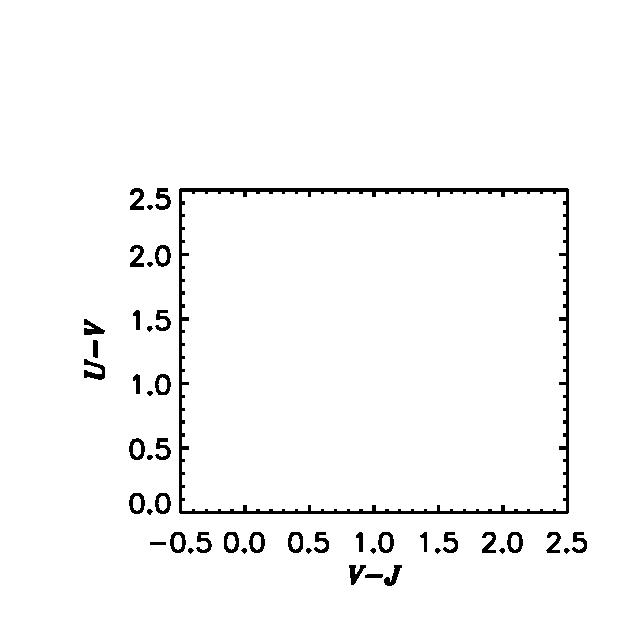
\includegraphics[width = \columnwidth, trim=1cm 0.7cm 0cm 3cm]{context}
	\caption{\bfb Some heuristic/contextual map of the sample data to orient the reader: UVJ plot, 
			$\Mstel$ histogram, half-mass time histogram, or all of the above. I don't want to 
			clutter any of the subsequent plots with this stuff.}
	\label{fig:sample}
\end{figure}

%------------------------------------------------------------------------------------------------------------------------------------------
%------------------------------------------------------------------------------------------------------------------------------------------

\begin{figure*}
	\centering
	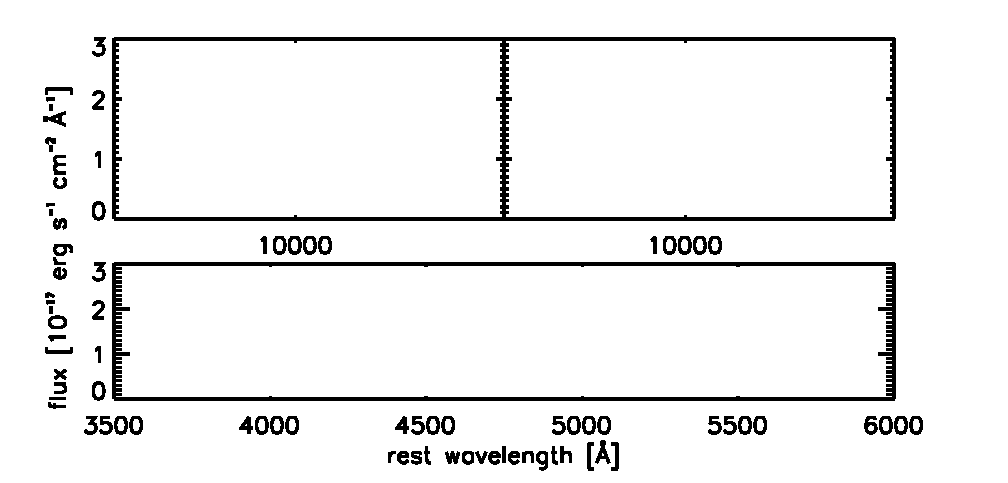
\includegraphics[width=0.85\textwidth]{scheme}
	\caption{\bfb A 3-panel figure---2 top + 1 bottom. At top, show D18-like figures of the CSI
			data + SFH reconstructions for one object. I don't think we need to show the spectral
			sub-components for the chunky fit; just the best fit low-res SED and SFH. Other parameters
			at Dan's discretion, but they shouldn't clutter anything up; the key is the low-res SED.
			At bottom, show the full IMACS high-res spectrum for the same object and overlay the
			matched-resolution predictions from both SFH reconstruction techniques. Whatever
			colors we use here we'll stick with for the rest of the paper. The object probably should
			be like SA-type; nice absorption, some emission.}
	\label{fig:scheme}
\end{figure*}

\begin{figure}
	\centering
	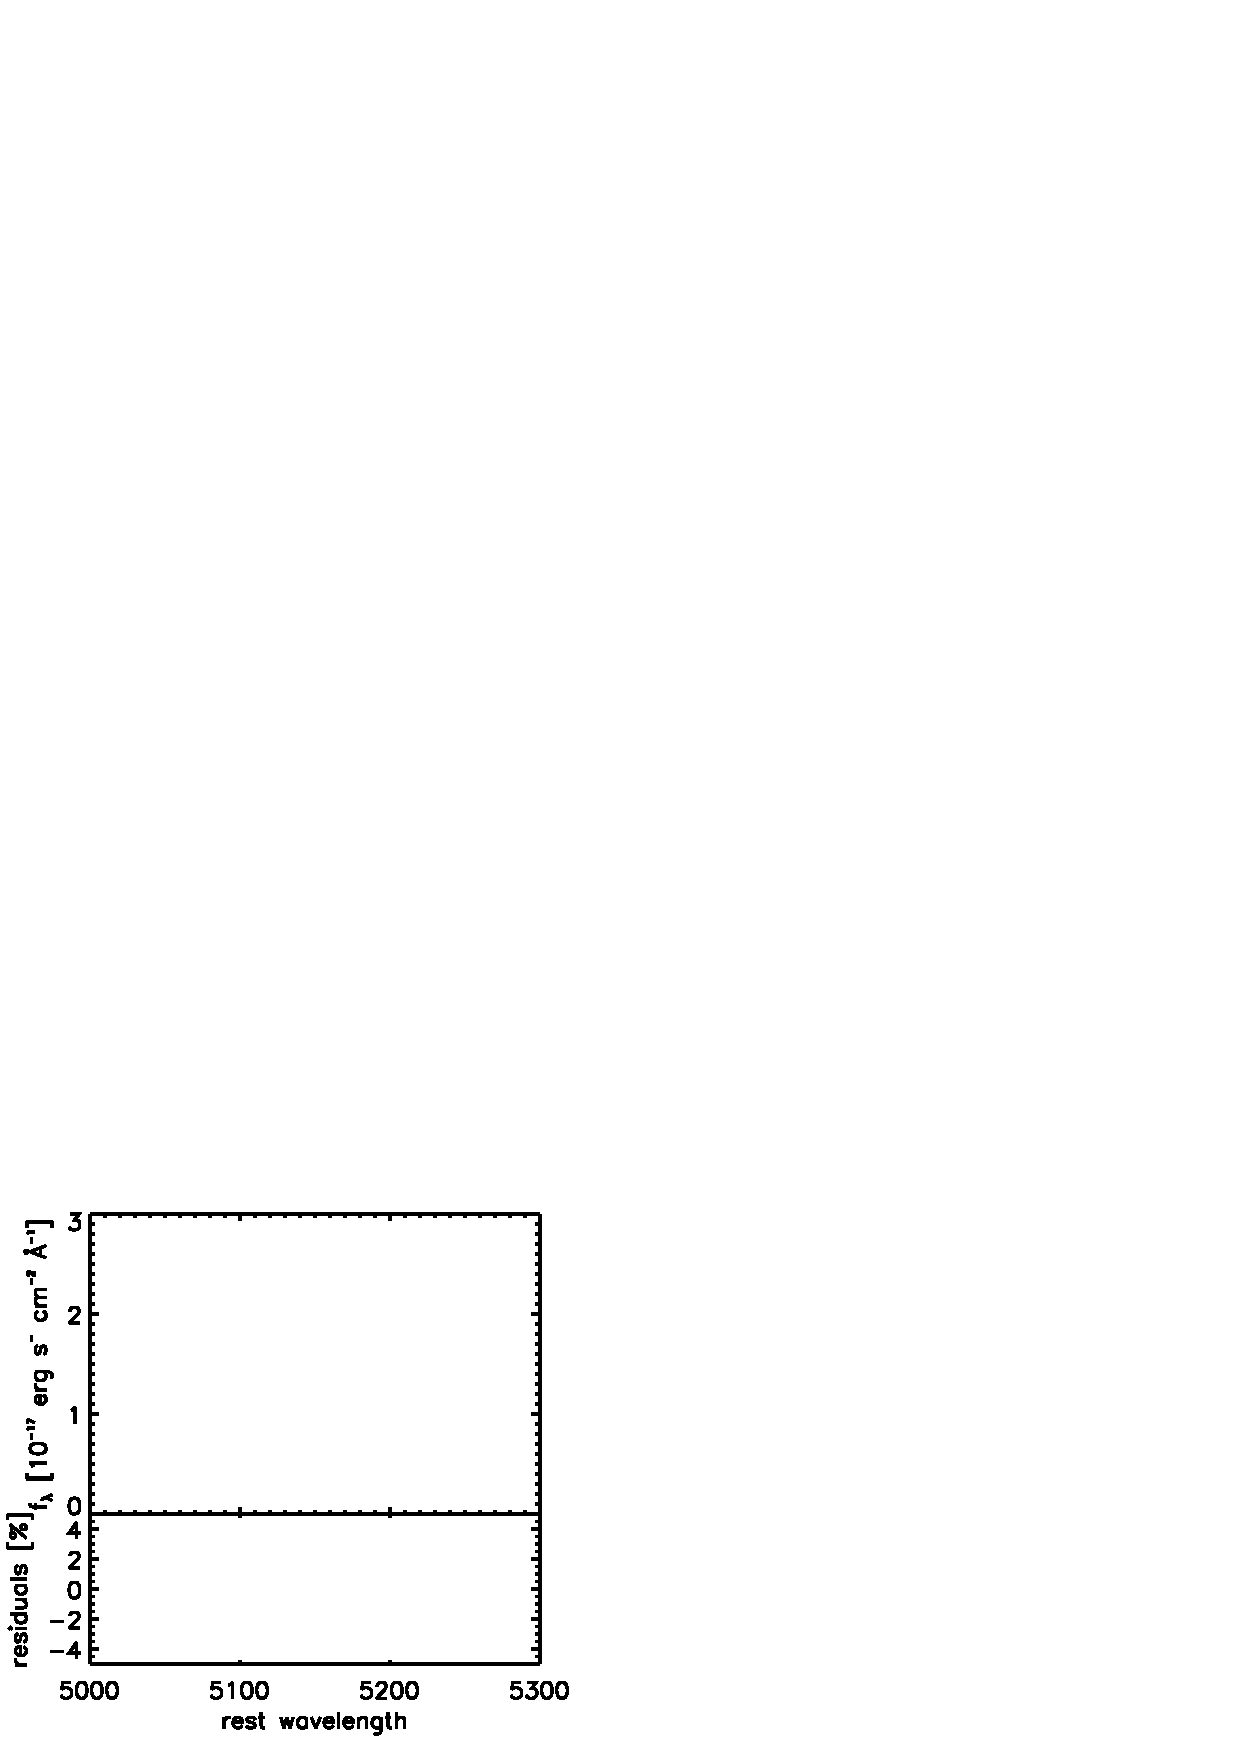
\includegraphics[width = \columnwidth, trim = 0cm 0.7cm 0cm 0cm]{metric}
	\caption{\bfb A graphic example of how we calculate whatever residuals we illustrate
			in Figure \ref{fig:resids}. Could be 2 panels, one showing the raw line + model,
			another showing the residuals. Could be 1 panel split in half. Could be for one
			object, or the full sample with the average models overlaid. Can just pick one
			SFH technique.}
	\label{fig:metric}
\end{figure}

\section{Results}
\label{sec:results}

Here we compare the model high resolution spectra generated from the SFHs inferred using 
Techniques 1 and 2 (Sections \ref{sec:blocks}, \ref{sec:h1}) to actual high resolution spectra taken for
the same objects. In all but one case, we find that the median predicted line strength is within 
1\% of the measured value. 

We study the model spectrum corresponding to
the maximum-likelihood SFH fit. Uncertainties are tabulated for the SFHs and attendant 
parameters, but not propagated to the high resolution spectral models. As such,
the comparisons below treat the predictions as more credible than they are. Combined with the fact 
that the model metallicities are age-independent, our experiment is biased towards 
revealing significant differences between the data and the predictions. Any offsets we find---in units
of flux or standard deviations---are thus closer to upper limits. %: the latter are less flexible than they could be and given greater credence than they should be.

{\bfb LEA -- some note here about whether we're going to focus on the full spectrum or just the ``line
strengths.'' The latter is justified because it's the real value-add of the high-res data, and also because
I assume the same photometry was used to flux both the prism data and the high-res spectra. We
just have to explain it.}


%%%
%%%

\begin{table*}
	\centering
	\caption{Summary of experimental results. Mean equivalent widths are quoted for the full sample.
			{\bfr Asterisks denote feature outside the CSI prism wavelength coverage.}}
	\label{tbl:stats}
	\begin{tabular}{cccccccccc} % four columns, alignment for each
		\hline
	Feature & Band center [\AA] & Bandwidth [\AA] & $\langle{\rm EW}\rangle$ [\AA] & 
	\multicolumn{2}{c}{Full sample offset [\%]} & 
	\multicolumn{2}{c}{{\bfr Red} sample offset [\%]} & 
	\multicolumn{2}{c}{{\bfr Blue} sample offset [\%]}\\
	& & & & Tech.~1 & Tech.~2 & Tech.~1 & Tech.~2 & Tech.~1 & Tech.~2\\
		\hline
	CaHK & {\bfr LAMBDA} & {\bfr LAMBDA}\\
	CN$_{1}$    & 4159 & 35 & foo & foo & foo & foo & foo & foo & foo \\
	Ca4227 & 4228 & 12\\
	G4300  & 4298 & 35\\
%	Fe4383 & 4394 & 51\\
%	Ca4455 & 4463 & 22\\
	Fe4531 & 4536 & 45\\
	C$_{2}$ 4668 & 4677 & 86\\
%	Fe5015 & 5015 & 76\\
	Mg{\it b}    & 5176 & 32\\
	Fe5270 & 5265 & 40\\
	Fe5335 & 5332 & 40\\
%	Fe5406 & 5401 & 27\\
%	Fe5709 & 5708 & 23\\
%	Fe5782 & 5786 & 20\\
%	Na     & 5893 & 32\\
%	cn2    & 4159 & 35\\
%	mg1    & 5101 & 65\\
%	mg2    & 5175 & 42\\
		\hline
	H$\delta_{\rm A}$    & 4102 & 38\\
	H$\gamma_{\rm A}$    & 4341 & 43\\
	H$\beta$     & 4862 & 28\\
%	hdf    & 4101 & 21\\
%	hgf    & 4341 & 21\\
		\hline
	\end{tabular}
\end{table*}

%%%
%%%

\begin{figure*}
\includegraphics[width = \textwidth]{residuals}
\includegraphics[width = \textwidth]{residuals}
\caption{\bfb Main plot, only the absorption features (no Balmers), Technique 1 at top and 2 below.
		I think we should look at versions highlighting any ranges outside the prism bandpass 
		(at the median or $N$th percentile redshift or whatever) and also see what happens when
		the individual residuals are lightly traced in grey or something. We also need to determine
		how we'll split the data (UVJ or (N)LB); if we go w/ UVJ perhaps we can add the LB/NLB
		version in an Appendix. I think we should also shrink the vertical scale to $\pm$5\%.}
\label{fig:resids}
\end{figure*}

\subsection{Experimental setup}
\label{sec:setup}

Figure \ref{fig:scheme} outlines the experiment. The {\bfr top} panels show the
CSI spectrophotometry for a galaxy at redshift {\bfr ZZZ}, along with its inferred SFH using Technique 
1 (left) and 2 (right). The CSI data have broad wavelength 
coverage and dense but coarse sampling over the rest optical. As such, they reflect a relatively
complete accounting of a galaxy's stellar photospheric continuum emission. With the exception of the
strongest/broadest absorption features---e.g., H$\beta$; the Mg $\lambda$5170 triplet---these data are 
insensitive to absorption lines and any historical information they might convey.

Figure \ref{fig:scheme}, {\bfr bottom}, shows the complete high resolution IMACS spectrum of 
this object with the matched-resolution spectral predictions from the SFHs in the top panels overlaid. 
Results from Techniques 1 and 2 are in {\bfr color 1} and {\bfr color 2}, \resp. 

The data in the two top panels are identical; only the models change from left to right. Likewise,
both model predictions are compared to the same $R\sim800$ IMACS data. We therefore perform two 
experiments in parallel, identical except for the method from which the high resolution prediction is 
generated. {\bfr We comment on the differences between the results from each
technique in Sections XYZ, but they are ancillary to our main point.}

Figure \ref{fig:metric} illustrates how we compare our spectral predictions to the high resolution data.
Here, we re-present Figure \ref{fig:scheme}, bottom, zoomed-in to the region surrounding {\bfr FEATURE}.
{\bfb LEA -- If we need to divide the data by the model, we'll make this 2 panels.} The central 
bandpass of the corresponding Lick index is shown in {\bfr however} (\CITE). We define 
the mismatch between prediction and high resolution data as:
\begin{equation}
	\bfr \Delta = {\rm whatever~Dan~says}.
\end{equation}
That is, a quoted difference of 5\% in a given spectral feature corresponds to {\bfr whatever per-angstrom
offset integrated over however many angstroms, or whatever Dan did.}

We then compute {\bfr$\Delta$} for each Lick bandpass in each galaxy.

{\bfb LEA -- Here is where we talk about limiting ourselves to a comparison in the lines or mention
that we calculate global $\chi^{2}$ values and point to where we'll discuss those.}

\subsection{Sample-wide outcomes}
\label{sec:upshot}

Figure \ref{fig:resids} and Table \ref{tbl:stats} summarize the quality of our model predictions 
across the entire \ntot\ object sample; i.e., the overall outcome of our experiment. In the figure, 
results from Techniques 1 and 2 are shown in the top and bottom panels, \resp. At the central 
wavelength of each feature, we show the median, 16th, and 84th percentile offsets in a given sample. 
Results based on the full sample are shown in black, with red and blue boxes denoting 
{\bfr SFR-defined} subsamples, \resp. The width of each box corresponds to the width of 
that feature's Lick bandpass. Regimes outside the original prism wavelength range are highlighted 
{\bfr in some color}. The dashed and dotted horizontal lines \resp\ benchmark mismatches at the 
$\pm$1\% and $\pm$2\% level.

Clearly, {\it almost all rest-optical galaxy absorption features 
visible at $R\sim800$ are predictable to better than 1\% by models tuned to data with $\sim$30$\times$
lower resolution} but broader wavelength coverage. That is, to a very high degree of accuracy, one can 
infer the strengths of nearly all major optical stellar absorption features in integrated galaxy light 
without ever detecting any of them.

This statement holds for any feature in any subsample except one. 
{\bfr State mean total offsets for both types (Table \ref{tbl:stats}).} It holds irrespective of the feature's 
width---{\bfr basic quantification}---and irrespective of the chemical species traced. 
It holds for strong features---e.g., the G band in passive objects {\bfr quote mean
EW}---and weak ones---e.g., Mg{\it b} in starforming ones {\bfr quote mean EW}. Simply: we 
knew the fluxes of each \AA ngstrom of our high resolution spectra before we got to the
telescope.

The lone exception is Ca4227 in {\bfr passive}, but not starforming galaxies. {\bfr Something 
about the history of this line being anomalous, Ca-rich supernovae, etc.} As CSI was designed 
to probe spatial overdensities, {\bfr
and some of these objects are for real in dense places?}, we believe the $\sim$2.5\%
mismatch we see here may reflect the same phenomenon. Regardless, this finding suggests either that
slightly different abundance patterns should be assumed when fitting passive objects (\CITE), 
or that Ca4227 strengths might be used to enhance SFH estimates. We touch on the latter in 
Section \ref{sec:discussion}, but note here that any prior would have to be accurate to better than 
2\% in the mean for this relationship to be useful.

\subsection{The Balmer lines}
\label{sec:balmer}

Figure \ref{fig:balmer} shows the same offset summaries as Figure \ref{fig:resids} but for the three
strong Balmer lines in the prism data: H$\delta$, H$\gamma$, and H$\beta$. {\bfb LEA -- we'll have 
to see what these look like. I don't think there's anything interesting to be said here, just to show that
the only sizeable discrepancies are readily attributable to emission. If it holds up, we can also make
a note about the enhanced performance of the $H=1$ models here versus the chunky fits.}

\begin{figure}
\centering
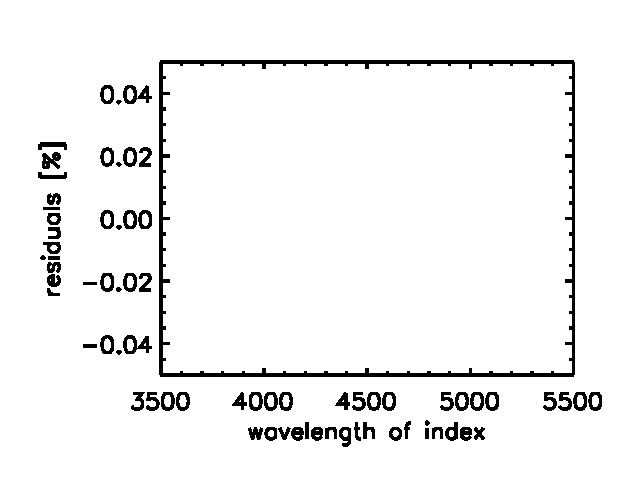
\includegraphics[scale = 0.9, trim = 1cm 0cm 0cm 0cm]{balmer}
\caption{\bfb Show the offsets for the Balmer line predictions; same styling as Figure \ref{fig:resids}.
		Can potentially add another panel for, e.g., H$\beta$ specifically showing the unmodelled 
		emission. Can also put this up in Figure \ref{fig:metric}, but I think best to bury it down here.}
\label{fig:balmer}
\end{figure}

\subsection{Systematic errors}
\label{sec:systematics}

The above comparisons are affected by {\bfr three} main systematics: redshift refinement, 
velocity broadening,
and continuum matching. 
%{\bfb (LEA -- Dan, is the latter the case? Are the high-res IMACS data fluxed
%to the same photometry as the prism data? Do we perform a 2nd order correction somewhere to take
%out any continuum mismatches pre-comparison? If so, we'll state that above where noted and cut any
%discussion from this section.)}

Regarding redshift refinement, both SFH inference techniques 
adopted discrete redshift steps of $0.005\leq\Delta z \leq 0.01$ (Section \ref{sec:data}). 
This interval was sufficient
given the low resolution of the CSI data, but the newer IMACS data allow for
more precision. As such, there are typically mismatches of 
{\bfr $\delta z \approx ZZZ$} between the predicted locations of spectral features and where they 
ultimately appear in the high resolution data.

Regarding velocity broadening, the CSI data are likewise too coarse to permit velocity
dispersion estimates. As such, the high resolution spectral predictions
must be broadened from the native FSPS resolution to whatever the $R\sim800$ IMACS data imply
for each object. 

We correct for both issues by {\bfr Dan to discuss how he shifts and broadens the models here}.

These offsets are important: they illustrate the only first-order orthogonal axes in the problem of SFH 
reconstruction: velocity and age. They also show us that higher resolution spectra add meaningful 
signal in Doppler---if not age---space. Unfortunately, it appears unlikely that independent Doppler
information can be exploited to enhance SFH estimates (Section \ref{sec:discussion}), but it
is nevertheless where having high resolution data is obviously helpful.
%{\bfb LEA -- the conclusion is that more pixels buy you velocity but not SFH stuff. 
%This is trivial: Doppler physics modify 1--10\,\AA\ scales, line strength physics are stellar 
%continuum physics and modify 1000--10,000\,\AA scales. We knew this: we knew that
%the continuum from [\ion{O}{ii}] to [\ion{O}{iii}] is linked 1:1 with the Balmer strengths. 
%It's this way for all lines (it's all opacity); BC03 tells you that, with enough precision on the 
%continuum, you have the same purchase on the metallicity as you would if you had all the 
%lines. This is true up to odd abundance patterns, which may or may not be useful as 
%SFH priors.}

\begin{figure}
\centering
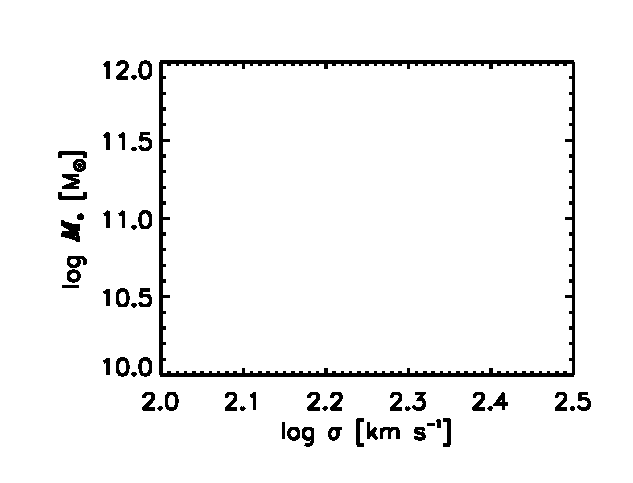
\includegraphics[scale = 0.9, trim = 1cm 0cm 0cm 0cm]{disp}
\caption{\bfb Show $\sigma$ distributions or $\sigma$--$\Mstel$ for LB/NLB objects.}
\label{fig:disp}
\end{figure}

The last systematic is mismatches in the stellar continuum. {\bfr Dan to send methods.}

\if0
Here's the way this should go:
\benum
	\item Show 1 example of CSI data, SFH inference, high resolution output. Overlay the H=1 and block
		results at high resolution on the IMACS spectrum. (Method walkthru; wavelength context.)
	\item Show an example of how the residuals are calculated. (Center of bandpass? Integrated EW
		difference? Mean offset across bandpass?)
	\item Show the summary residuals across the sameple. Show the breakdown by UVJ and age 
		(half mass time). 	Do this only for the absorption lines. Overlay H=1 and blocky results? Possibly use
		only one approach and discuss any offsets. If so, show all of the spectra? We'll want a comparison 
		plot (residuals v. residuals) for internal use. In the final plot, highlight any features that are 
		outside the 	prism bandpass.
	\item Panel and brief section (paragraph) about emission lines since there is a difference between
		the inferences. This figure is cuttable.
\eenum
\fi

%------------------------------------------------------------------------------------------------------------------------------------------
%------------------------------------------------------------------------------------------------------------------------------------------

\section{Discussion}
\label{sec:discussion}

%\benum
%	\item Need to have some plot and metric of the velocity dispersions for LBs and NLBs. Some
%		limit on whether these are inconsistent over fixed mass intervals.
%\eenum


\subsection{Implications for direct SFH inference}
\label{sec:sedMap}

Our experiments imply that high resolution optical spectroscopy of any quality reasonable
to expect for individual distant objects will not meaningfully 
enhance knowledge of their underlying stellar populations compared to much more coarsely and broadly 
sampled datasets (see Section \ref{sec:stacking}). That is, absorption line 
details---at least as presented at a galaxy's velocity dispersion---are sufficiently correlated to 
stellar continua on large scales that capturing the details 
of the latter across a long enough wavelength baseline yields the same information as 
densely sampling the rest optical. There is therefore no need to obtain 
costly, high resolution spectroscopy for SFH inferences.\footnote{A future 
paper will show that, at $z\sim0.4$, the 26-band UltraVista filter set \citep{Muzzin13} performs 
similarly to CSI, meaning that even the prism data used here is likely oversampled.}
{\bfr In this, we reinforce findings by \citet{Pacifici12}, who show that---limited to 
rest optical data---$R\sim1000$ spectra enhance SFH estimates less than other inferences 
compared $R\sim100$ spectra (25\% v. 45\% drops in uncertainty; see their Table 2).} 
We would add, however, that, had that study incorporated UV--IR photometry, 
those gains would have been reduced. {\bfb LEA -- \citep{Leja19, Lower20} show that once you have
the kind of coverage we have changing the SFH parameters modulate the high resolution
spectra at the 1\%--2\% level.}
Further insights into galaxy growth will not be gleaned by adding better spectra, but rather
from the methods and results that reveal why that statement is true.

This lesson is not new. The fact that 
metallicity modulates continuum light on $\sim$100--1000\,\AA\ scales is apparent in the
output of any stellar population synthesis code. The phenomenon is also well recognized in 
some contexts, such as as the tracking of Balmer line depths with $U-B$ or D4000 
\citep[e.g.,][]{Kauffmann03,CidFernandes05}. What we have shown is simply that the above is true---perhaps
to a greater than expected extent---for all (Lick) species. The observational trick is to sample the 
SED so as to capture all of the relevant signal at minimal cost. We do not know the optimal sampling,
 only that CSI apparently meets the criteria that define it.

Nevertheless, these findings reinforce or suggest practical, informatic, and 
theoretical programs that we believe will be more informative than simply taking more or
``better'' data.

\subsubsection{Practical}

The practical upshot of the above is twofold. First, there is no need to expend telescope
or computer time obtaining and modeling thousands of SED points for the purpose of inferring 
galaxy growth. Second, on the modeling side, the physical correlations between spectral
elements should be accounted for mathematically to avoid drawing inferences of unreasonable 
certainty. Each pixel may be formally independent, but it does not add a new degree of freedom.
{\bfb LEA -- this is the place to discuss previous work on or findings to this effect. The fact
that $S/N$ doesn't really matter has been noted in a bunch of places before, e.g., \citet{Leja19}.
We disagree with those authors about the utility of adding bedder spectra---even though they
see similar offsets to us (2\%; their Figure 8)---but may agree with \citet{Ocvirk06} about it?

The narrative here is something like: limited to the rest optical, Pacifici showed there's only
marginal gains from going to R=1000 spectra for SFH inferences vs R=100. Leja showed that, 
using UV--IR photometry, $S/N$ doesn't matter for SFH inferences. We do something like
combine the two: if you have sufficiently broad SED sampling, the SFHs you infer are good enough
to remove any reason for $S/N$ or resolution to matter because all of the information those
things could add has been accounted for.

Also, we're working at about 1/2 the age of the universe at least compared to Camilla, if not
Leja, too.}

\subsubsection{Informatic}

The informatic upshot of the above is that there exists a data compression scheme---a way to
distill covariant pixels to independent degrees of freedom---that may be
worth identifying if SFH inferences for large samples is to play a substantial role in extragalactic 
astronomy's future. Given the deluge of SEDs that PFS, LSST, and WFIRST will soon deliver, 
modeling efficiency will be critical to characterising representative swaths of those datasets. 
It is likely that such a compression scheme will resemble what intuition
and, e.g., CSI suggests: sparse UV and IR sampling with finer---but not fine---sampling over
the rest optical, particularly from around the Balmer break to around the magnesium triplet,
where intermediate age stars make the greatest impression \citep[e.g.,][]{Dressler16}. However,
it is also possible it will not resemble that configuration, so we encourage serious work on this 
issue ({\bfr or cite and amplify}).

\subsubsection{Theoretical}

The theoretical upshot is that understanding this compression scheme---even if it is as basic 
as the above---represents understanding the extent to which information about the
physics an object was subject to over its history could possibly modulate its presentation at the one epoch we 
will ever witness it at. That is, it must reveal the bedrock of the SFH $\mapsto$ SED mapping, and 
therefore something close to the epistemological ceiling for the study of galaxy evolution. Knowledge 
of that boundary condition cannot but enhance the questions investigators ask and the investigations 
they pursue. Given the substantial human and technological resources devoted to such endeavors, 
that insight seems beneficial.

How mechanically to reverse engineer this compression scheme is a separate question. Machine learning 
could be used to identify via simulation the hypersurface characterising the precision to which 
$\Mstel(t)$ is knowable as a function of data---$S/N$, SED sampling---and galaxy 
properties---$z$, $\ssfr$, $Z$, $\sigma$, $A_{V}$, environment, morphology. A simpler exercise,
is simply to invert the experiment we performed, fitting SFHs only to high resolution optical 
spectra and predicting broadband fluxes the blue and red. One could then repeat this exercise 
downgrading the resolution or omitting portions of the starting spectrum and measuring how 
the extrapolations changed, adding outrigger photometry as soon as the predictions began to deviate
significantly from the truth. Figures 12 and D2 of \citet{Abramson20} show an examples of this kind of 
approach---and hint at the predictive quality as a function of SED type---which of 
course could also be coupled to machine learning.

%fits to
%low resolution rest-optical spectra like those from CSI do not predict, e.g., infrared
%broadband fluxes to the level the high resolution lines are reproduced here, but they
%do quite well in some systems. Of course, this exercise could also be coupled to machine learning.

Based on our results, however, similar exercises performed using only photometry 
(Abramson in preparation), and the physics at play, we suspect that full UV--IR 
wavelength coverage will be one of the foundations whatever map is finally produced: If all of 
the starlight is captured, the density of the sampling is secondary (provided it is sufficient
to obtain accurate redshifts). Future surveys designed to support SFH reconstruction should 
therefore opt for increased wavelength coverage at the expense of SED resolution. 
%It may remain easier to take multiplexed prism spectra 
%than a dozen bands worth of photometry, but it probably still represent oversampling.

%We suspect 
%that wavelength baseline is the underlying key to SED fitting. To test this, one could derive
%SFHs based on fits to the high resolution spectra presented here and try to predict the broadband
%fluxes well outside the rest optical. 

% The outcome of
%this test using high resolution spectra as a starting point would inform us as to the relative
%priority of broad baseline photometry vs deep spectroscopy in the study of galaxy growth. 
%{\bfr This is crap; you always need a redshift and I think ultimately that's the trick.}

%line information is determined by some (unknown) combination of the local and remote 
%continuum. 

%We already knew this: we knew that
%the continuum from [\ion{O}{ii}] to [\ion{O}{iii}] is linked 1:1 with the Balmer line strengths. 
%Of course, it's this way for all lines (it's all opacity), and BC03 tells you that, if you have enough
%precision on the continuum, you have the same purchase on the metallicity as you would if you 
%had all the lines. 

Of course, we are not asserting that there is never a reason to take high resolution spectra. If 
one is interested in the IMF \citep{Conroy12}, specific abundance patterns, or kinematics, it is 
clearly necessary. We only argue that it seems very unlikely that these investigations will
qualitatively enhance assessments of galaxy growth.

The only avenue we have found where they might is calcium strengths. These seem to 
add a relatively large amount of information to our predictions in passive galaxies compared
to the other Lick indices. However, while the prediction/data mismatches are indeed twice the 
average offset, they are still only at the 2\% level. As such, to enhance SFH predictions, priors 
linking Ca abundance to age must be accurate to at least that level, and spectra must have 
$S/N\gtrsim14\,\AA^{-1}$ to see the signal at $1\,\sigma$. We believe attempting to construct 
such an object or take such data are endeavors of diminishing returns: aperture and other 
observational effects surely distort one's ability to interpret such precision when present, 
and---as in the case of calcium---other, more easily observed properties like environmental 
density (\CITE) are almost certainly equally good candidates for an age prior.

\begin{figure}
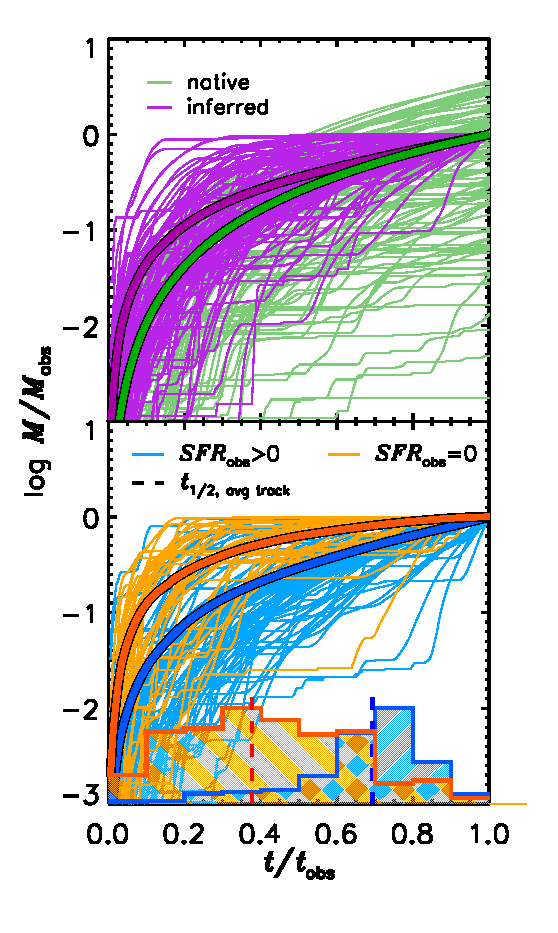
\includegraphics[trim = 0cm 1cm 0cm 0cm]{noStackShowV}
\caption{\bfb LEA -- here's why stacking will not buy you much. The difference between
		the various half mass time averages is $\sim$2\%--3\%. I'm not sure if that matters
		but I calculated it.}
\label{fig:noStack}
\end{figure}

\subsubsection{What about stacking?}
\label{sec:stacking}

It is reasonable to think that, while $\sim$1\%--2\% line strength precision is unobtainable for 
useful numbers of individual objects, stacking can easily achieve that $S/N$ (\CITE), and the stacks 
can be modeled to infer the average growth trajectory of the constituent objects. Mathematically, this
is of course true, but two examples illustrate why that statement is unhelpful for physics.

Figure \ref{fig:noStack} explores different kinds of $H=1$ SFH ensembles---i.e., the prior behind
Technique 2 SFH inferences (Section \ref{sec:h1}). These are similar to, e.g., the suite of semi-analytic
model-derived histories used by \citet{Pacifici12}. 

The top panel shows in green the native distribution of mass growth trajectories modeled forward 
from $t=0$ to $t=1=\tobs$ with the ensemble's  {\it mean} mass normalized to $\langle M\rangle=1$ at $\tobs$. 
Overlaid in purple is exactly the same distribution of SFHs, but normalized such that {\it each track} 
has $M=1$ at that time. The latter tracks are what actually go into the fitting---each track in the library 
normalized to a small range of masses based on the luminosity and color of the object---and the inferred 
mean history derived therefrom is significantly different from the native mean trajectory. This 
difference between mean histories is the measurement needed to assess whether $H=1$ is the correct
SFH reference set. It is derived from a stack of histories, not having good precision on one track,
and therefore doesn't need high precision data to be ascertained. {\bfb LEA -- I think I'm gonna cut this.}

The bottom panel shows more intuitively why stacking is unhelpful. There, we reproduce the pink
tracks from the top panel, but split them into those tracks that are passive (orange) or starforming (blue)
at the epoch of observation. At the bottom, we plot the distribution of half-mass times for each subsample.
From these, it is clear that a stack based on objects of the same stellar mass and SFR---intuitive classes
to average over---might contain objects with half-mass times that differ by 40\% of a Hubble time.
What the average of these tracks---at any precision---would tell you about the physics that caused any 
one of them to behave as it did is hard to see.

The trouble is that, physically, what is of interest is and only is either (1) a high-fidelity assessment of 
the SFHs of individual objects, or (2) the {\it typical SFH} of a meaningfully defined class of galaxies. 
It is not clear that (2) is derivable from (1), because ``typical'' in this sense should properly refer to the 
{\it mode} history---that which the largest number of class members experienced---not the {\it mean},
but, if the latter is our only proxy for the former, it is certainly assessable by averaging over many low-fidelity
assessments for individual objects. I.e., a stack of the {\it histories}, which doesn't require good data. This
is what Figure \ref{fig:noStack}, bottom, shows.

Whether you can actually derive such a meaningful class is questionable because observed properties
are poor proxies for historical ones (bottom), but, if you could, again the physics is in the difference
between forward and backward projected SFH inferences (top). 

For neither purpose is high-precision high resolution spectra beneficial.

%{\bfr Something about why it's not going to help to stack a bunch of objects to get $S/N\sim100$
%in some average. *Maybe* a plot on the fact that you can only ever group things by where they 
%appear, not where they start, which means you never really know what the output represents. See
%noStackShow.eps}

%This fact prompts three questions: (1) Why? (2) What are the extra pixels doing? (3) What does
%this mean for the future? All of these relate to the difference between formal and meaningful 
%information content.

%The nature of this correlation is the mathematical key to understanding the SFH$\,\mapsto\,$SED 
%mapping, and therefore our ability to invert the latter to get at the former; i.e., execute an empirical 
%study of galaxy evolution.

\if0
In the immediate term, the upshot is that suitably sampled SEDs need never be well sampled, at least
not to understand mass growth (Section \ref{sec:redshifts}). What ``suitable'' means would be determined 
by the above investigation, but clearly CSI meets or exceeds that threshold at $z\lesssim1$.\footnote{A future 
paper will show that the 26-band UltraVista filter set \citep{Muzzin13} probably also does as well at 
$z\sim0.4$.} Of course, this implies that many current (and future; Section \ref{sec:future}) data sets 
are oversampled, and that it is inadvisable to use those for SFH modeling while assuming that each 
pixel adds one degree of freedom. Adding systematics that correlate pixels is a minimum requirement 
to reinflate the resultant SFH uncertainties, but a floor will ultimately be necessary. It is very possible 
that we have already reached that floor.
\fi

% in terms of the number/span of bandpasses required to 
%predict SFHs to a given precision as a function of redshift 
%though it is very different from the question of ``What is a galaxy's SFH?'' 

\subsection{Prospects for exploiting Doppler information}
\label{sec:redshifts}

The area where high resolution spectroscopy yields unique insight is velocity space. The 
obvious enhancement is to redshifts. This may be important to mitigate against, e.g., [\ion{O}{ii}]
emission masquerading as an enhanced Balmer break at low resolution, biasing galaxy ages 
toward those of A stars. However, a more potentially useful application for SFH reconstruction
is through using kinematics inferred from line profiles.

It's tempting to contemplate using velocity dispersions 
to place colour-independent total stellar mass priors on SED fits to data of any resolution. This
move is especially appealing because it would provide a handle on faint/old stars that might imprint on 
a galaxy's velocity dispersion but remain undetectable in its SED. Unfortunately, a number of 
complications suggest that doing so would not significantly improve current methods.

The prior would most readily enter through a $\sigma$--$\Mstel$ relation. The intrinsic scatter
of this relation is $\sim$0.2 dex (\CITE), much broader than the formal---or even systematic---errors 
on SED-inferred stellar masses ({\bfr quote what we find; systematics as cross-method or duplicate
obs differences}). Further, that relation would be calibrated to stellar masses suffering the same 
systematic errors one wishes to correct by using the relation. Theoretically, a $\sigma$--S\'{e}rsic 
index--color relation---or some equivalent structure---could be used, but this entails other issues 
regarding spatial resolution, aperture matching, and dust effects. Finally, due, e.g., to inside-out 
growth (\CITE) and the existence of thick disks, each stellar subpopulation may contribute its own velocity 
dispersion to the global profile. If so, modeling dispersions will re-introduce exactly that the same 
degeneracies in line decomposition as arose with SEDs. These 
effects would have to be marginalized over---negating the precision gains---or the systematics from 
failing to do so would have to be understood.

{\bfr UTILITY AFTER SELECTION BY SFH---} Figure \ref{fig:disp} illustrates the sample's 
velocity dispersion estimates. Here, we show {\bfr what we show} for galaxies split by their inferred 
growth histories. {\bfr LBs show behavior X while NLBs show behavior Y.} %While more data is 
needed to say for certain, these trends suggest a link
%between age and velocity dispersion may provide a new and useful lever for SFH inferences.


We are bearish on the ultimate utility of kinematic stellar mass constraints, 
but we also do not know of any SFH modeling that has attempted to incorporate it. A 
study assessing its practicality and real-word effects would be edifying.

{\bfr NIRSPEC no good for SFHs but ok for kinematics + environments. Cosmology.}

%
%We now discuss these points in turn.
%
%The explicit science motivator for this study was inferring SFH, and, to a lesser extent, galaxy 
%enrichment histories, which we have shown are consistent with flat to {\bfr XXX\%}. However, 
%these are not the only applications for high resolution spectroscopy, and it is in the Doppler
%domain where the extra pixels play a key role.
%
%Redshift assessment is the obvious example. We discussed the average redshift offset between
%our low resolution inferences and high resolution data in Section \ref{sec:systematics}. It is
%doubtful that SFH properties covary with redshift errors at that level in general, but it may in 
%some cases. At CSI's spectral resolution, for example, [\ion{O}{ii}] $\lambda 3727$ is 
%almost indistinguishable from the Balmer break. While the break has substantial leverage 
%on the SFH, [\ion{O}{ii}] has none. Aliasing the line as a break would inflate the number 
%of A stars above what is real and bias the SFH inference towards that age range. 
%
%We do not 
%find this to be a problem ({\bfr see Figures XXX?}), but were also able to perform accurate
%emission line modeling. That may not be the possible in ever more ubiquitous slitless 
%spectroscopy from HST and JWST, and so may be more a problem in the future.
%
%Velocity dispersion are the more interesting example. High resolution is clearly needed to
%accurately infer this information, and it is indirectly related to the SFH through a galaxy's
%total stellar mass. Indeed, in principle, absent lensing, velocity dispersions are the only
%colour-independent mass estimators available. They are thus potentially powerful constraints
%even when their uncertainties are large.
%

%We are unaware of any SFH modeling that has incorporated or applied such a prior, but
%it should be explored. Unfortunately, at {\bfr 0.2 dex?}, the relation is probably not tight 
%enough to be decisive, but, if colour or structural subclasses are considered---it may help. 

%Principle among these in terms of SFH reconstruction is the determination of redshift. At high 
%resolution, the available number
%of constraining features is much higher than in the CSI data. {\bfr Something about the average
%redshift offset we find, the need to allow that to re-float when moving the predictions, whether
%that level of jiggle was appropriately marginalzied over in the original SFH inference, and whether
%that mattered.} This means that redshift--SFH covariance is stronger than it needs to be, inflating 
%the uncertainties on the latter. Furthermore, the added uncertainty comes in key places: 

%{\bfr A paragraph on the trivial cases of emission lines and IMF?}

\if 0
The trivial instance of this is in measuring emission lines, where resolution is needed to 
identify, e.g., embedded Balmer lines and detect subtle features like [\ion{O}{iii}] 
$\lambda4363$ ({\bfr cite Sanders}). Especially at low $S/N$, each pixel definitely counts
for these applications, and estimates of, e.g., nebular extinction, ISM metallicity, or outflow
properties will improve with every additional datum.

A yet more pertinent use would be to constrain the IMF \citep{Conroy12}. While doing so 
would have no bearing on the relative accuracies of SFH inferences, it would allow all stellar 
masses to be placed on a firmer absolute scale, which should enhance these objects power to test 
simulations or first-principles theoretical predictions. %Of course, if the IMF is allowed to vary with 
%time, one encounters the same problems as with $\sigma$.
%Redshifts, velocity dispersions, emission line details.
\fi

%\subsection{Future work}
%\label{sec:future}
%
%{\it Don't use JWST to take high resolution spectroscopy if you're interested in stellar mass growth!}

%------------------------------------------------------------------------------------------------------------------------------------------
%------------------------------------------------------------------------------------------------------------------------------------------

\section{Summary}
\label{sec:summary}

In the context of SFH reconstruction from full spectral fitting: high resolution doesn't buy you
anything new.

\bitem
	\item You can predict line strengths to 1\% without measuring them.
	\item Wavelength coverage beats spectral resolution.
	\item Metal enrichment histories for at least our sample are consistent 
		with flat to whatever corresponds to 1\% differences in line strengths.
	\item The goal is not to fit SFHs to SEDs, but to understand the sampling/compression
		scheme that enabled us to find what we found. This is the SFH$\mapsto$SED
		mapping and is equivalent to understanding the epistemological ceiling 
		in the study of galaxy evolution.
\eitem


\noindent\facilities\ Magellan/IMACS

\noindent\software\ Python (\texttt{CarPy}).%IDL (Coyote libraries; \url{http://www.idlcoyote.com/})

%------------------------------------------------------------------------------------------------------------------------------------------
%------------------------------------------------------------------------------------------------------------------------------------------

\section*{Acknowledgements}
LEA thanks Dr.~Lindsay Young for allowing him to find a place to write this text.

%------------------------------------------------------------------------------------------------------------------------------------------
%------------------------------------------------------------------------------------------------------------------------------------------

%%%%%%%%%%%%%%%%%%%% REFERENCES %%%%%%%%%%%%%%%%%%

% The best way to enter references is to use BibTeX:

\bibliographystyle{mnras}
\bibliography{/Users/labramson/lit} % if your bibtex file is called example.bib


% Alternatively you could enter them by hand, like this:
% This method is tedious and prone to error if you have lots of references
%\begin{thebibliography}{99}
%\bibitem[\protect\citeauthoryear{Author}{2012}]{Author2012}
%Author A.~N., 2013, Journal of Improbable Astronomy, 1, 1
%\bibitem[\protect\citeauthoryear{Others}{2013}]{Others2013}
%Others S., 2012, Journal of Interesting Stuff, 17, 198
%\end{thebibliography}

%%%%%%%%%%%%%%%%%%%%%%%%%%%%%%%%%%%%%%%%%%%%%%%%%%

%%%%%%%%%%%%%%%%% APPENDICES %%%%%%%%%%%%%%%%%%%%%

%\appendix
%\label{sec:appendix}

%%%%%%%%%%%%%%%%%%%%%%%%%%%%%%%%%%%%%%%%%%%%%%%%%%


% Don't change these lines
\bsp	% typesetting comment
\label{lastpage}
\end{document}

% End of mnras_template.tex